
\newboolean{setexpansion}
\setboolean{setexpansion}{false}

\newcommand{\cardborder}{
	\ifthenelse{\boolean{setexpansion}}{\expansion}{} 
	\purecardborder{}
}



%%%   Rules and additionals   %%%
\newcommand{\harborrule}{
	\begin{tikzpicture}
	\cardRuleImg{img/rules/harborLarge.png}
	%		\cardtypeItem
	%        \cardtypeAbility
	%		\cardtypeTest
	%		\cardtypeCharacter
	\cardtitle{Placement of harbor-tiles}
	\carddescriptor{Each harbor tile should be placed every other full tile apart. At a tile with two connecting edges the harbors should be placed facing inwards towards the center-most point.}
	%        \cardprice{35}
	\cardtypeRule{Set up}
	\cardborder
	\end{tikzpicture}
}

\newcommand{\setupGame}{
	\begin{tikzpicture}
% 	\cardRuleImg{img/rules/harbor2.png}

	\cardtitle{Setup for 1-4 \& 5-6 player game}
	\fulltikznode
	{
	    %% Tile images
	    {\centering
	    \begin{minipage}{.45\textwidth}
		    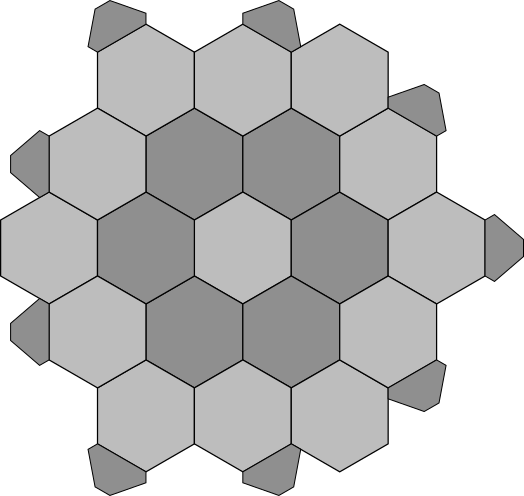
\includegraphics[width=\textwidth]{img/rules/small_build.png}
        \end{minipage}
        \hfill
        \begin{minipage}{.45\textwidth}
        \raggedleft
            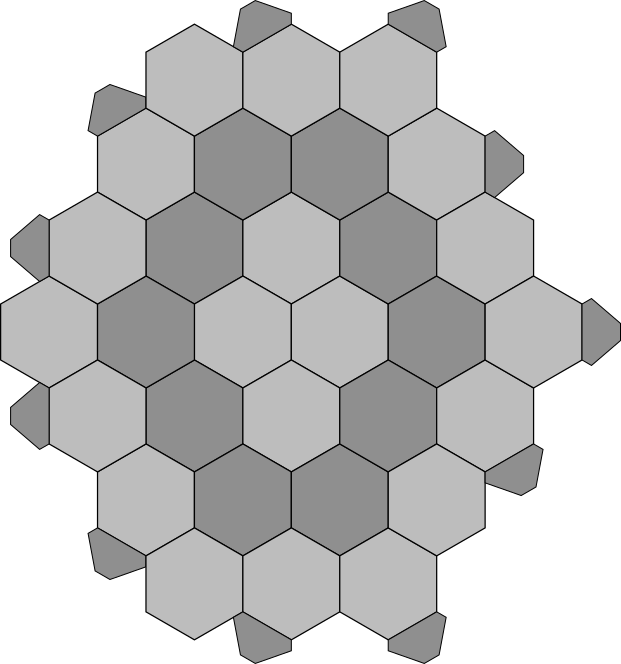
\includegraphics[width=\textwidth]{img/rules/large_build.png}
		  %  \fbox{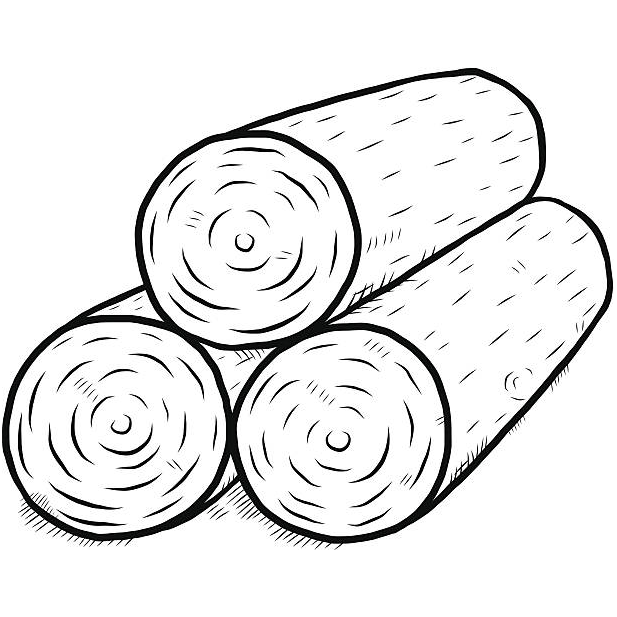
\includegraphics[height=0.6cm]{img/lumber.png}}
        \end{minipage}\\[30pt]
        }
	    
	    %% Description
	    \vrule width \textwidth height 2pt \\[10pt]
	    \footnotesize{
	        To set up a \textbf{(1-4 / 5-6)} player game follow the design from the illustrations above. \\
	        (Left: 1-4 players / Right: 5-6 players) \\[10pt]
	        Alternately, place \textbf{(5 / 6)} tiles in a horizontal line. Then, on each side place a new line with one tile less. Continue this pattern  until you place a \textbf{3} tile wide line on each side.\\[10pt]
	        Afterwards, follow the illustration on where to place the harbor tiles or follow the instruction on the relevant rule card.
	    }
	}
	
	\cardtypeRule{Set up}
	\cardborder
	\end{tikzpicture}
}

\newcommand{\setupNumberT}{
	\begin{tikzpicture}
% 	\cardRuleImg{img/rules/harbor2.png}

	\cardtitle{Setup Number tiles}
	\fulltikznode
	{
	    {
	    \centering
	    %% Tile images
	    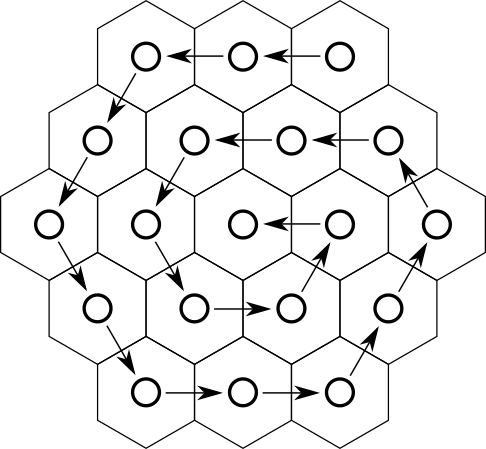
\includegraphics[width=.8\textwidth]{img/rules/numbers.png}\\[10pt]
	    }
	    %% Description
	    \vrule width \textwidth height 2pt \\[10pt]
	    \footnotesize{
	       % Place the number tiles with the letter side facing upwards. 
	        Start in an outside corner with the letter 'A' and continue placing the tokens in an alphabetical order, counter-clockwise towards the center of the board, skipping desert tiles.\\[10pt]
	        
	        Note that the 1-4 player game only have number tiles ranging [A-R] while 5-6 player game have [A-Zc]. Follow the correct letter while placing the tiles, for better control, place the letter-side up first and flip them when all tiles are correctly placed.
	    }
	}
	
	\cardtypeRule{Set up}
	\cardborder
	\end{tikzpicture}
}

\newcommand{\setupStart}{
	\begin{tikzpicture}
% 	\cardRuleImg{img/rules/harbor2.png}

	\cardtitle{Starting the game}
	\fulltikznode
	{
	   % {
	   % \centering
	   % %% Tile images
	   % 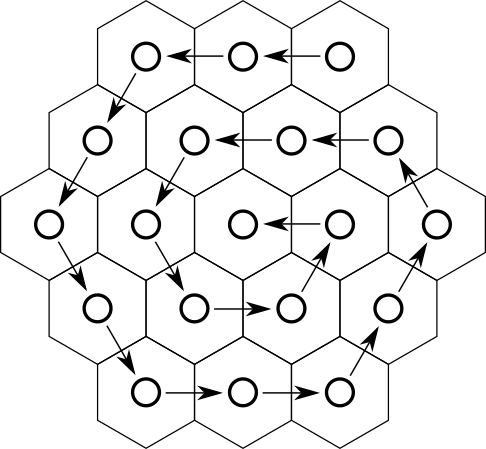
\includegraphics[width=.8\textwidth]{img/rules/numbers.png}\\[10pt]
	   % }
	    %% Description
	   % \vrule width \textwidth height 2pt \\[10pt]
	    \normalsize{%
	       During game start, the robber always starts in a desert.\\[10pt]
	       
	       The starting player is decided with a dice roll. All players in a clockwise order places one settlement at an intersection of their choice, along with one road connecting to the settlement. Afterwards the order is reversed, placing a second settlement and road at any location on the board.\\[10pt]
	       
	       \textbf{Note:}\\
	       The second road has to be placed connecting to the second settlement.\\
	       While the two initial settlements do not have to be placed connecting to each other, all settlements need to adhere to the rule of at least two road tiles apart.
	    }
	}
	
	\cardtypeRule{Set up}
	\cardborder
	\end{tikzpicture}
}

\newcommand{\ruleAddendum}{
	\begin{tikzpicture}
% 	\cardRuleImg{img/rules/harbor2.png}

	\cardtitle{5-6 p: The Special Build Phase}
	\fulltikznode
	{
	   % {
	   % \centering
	   % %% Tile images
	   % 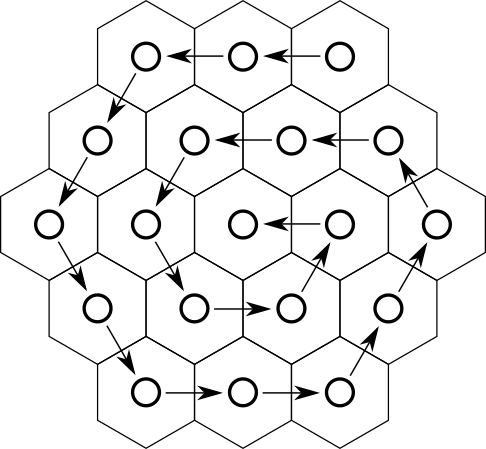
\includegraphics[width=.8\textwidth]{img/rules/numbers.png}\\[10pt]
	   % }
	    %% Description
	   % \vrule width \textwidth height 2pt \\[10pt]
	    \normalsize{%
	       With 5 or 6 players, after a player has ended their turn but before the next player roll the dice, there is the \textit{Special Build Phase}:\\[10pt]
	       
	       All the other players may participate in the special build phase. In clockwise order, each player then takes a special build turn. On your special build turn, you are allowed to build anything you can create with your resource cards, including buying development cards.\\[10pt]
	       \textbf{You are not allowed to} play development cards, nor do any kind of trading. You may only use the resources you have in your hand.\\[10pt]
	       
	       This gives the players a chance to avoid the robber and disrupt the other players, and encourages to trade as much and advantageously with the active player.
	   
	       
	    }
	}
	
	\cardtypeRule{5-6 player rule}
	\cardborder
	\end{tikzpicture}
}

\def\BCRuleSpace{5pt}
\newcommand{\buildcost}{
	\begin{tikzpicture}
% 	\carddebug
	\cardtitle{Building costs}
	\fulltikznode
	{
        %% Road
		\vrule width \textwidth height 2pt \\[\BCRuleSpace]
		\begin{minipage}{4cm}
		    \raggedright
            Road \\ \tiny{\quad = 0\enspace Victory Points}
        \end{minipage}
        \hfill
        \begin{minipage}{2cm}
        \raggedleft
            \fbox{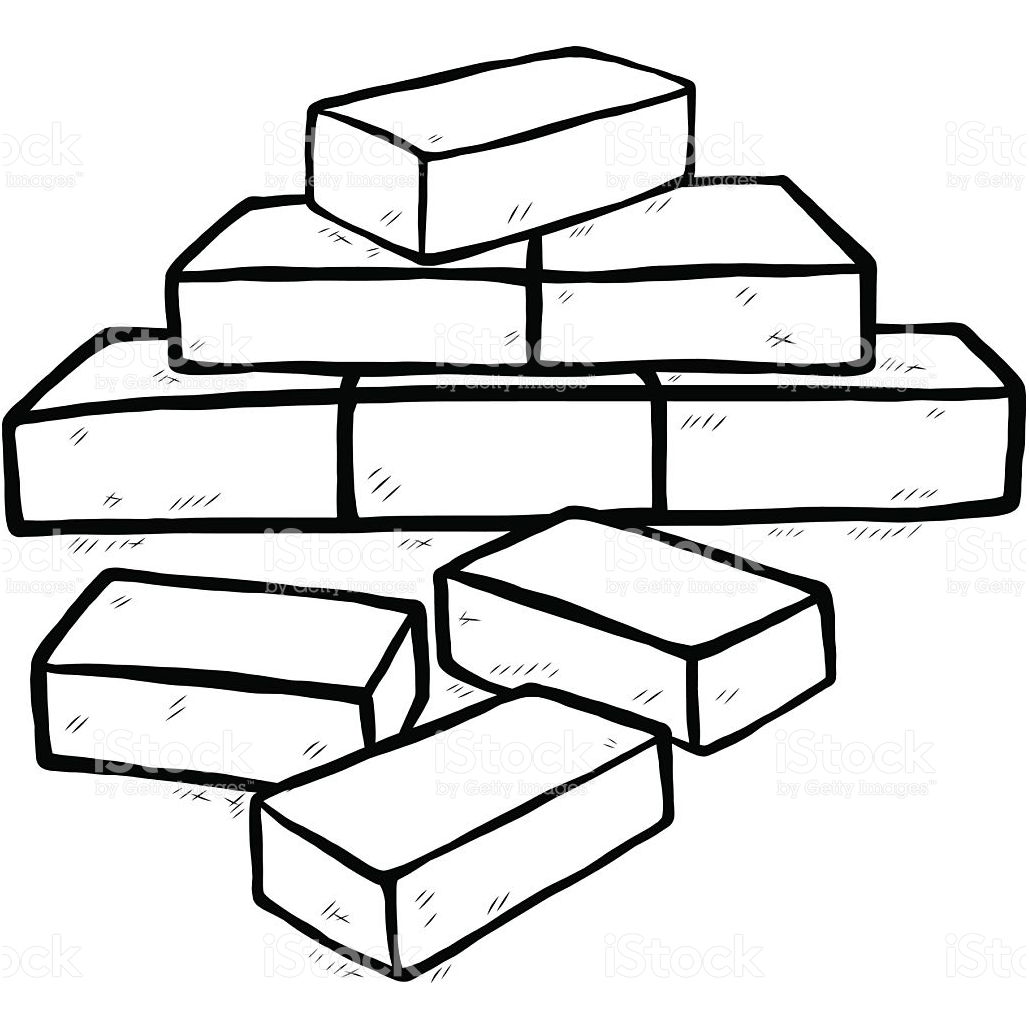
\includegraphics[height=0.6cm]{img/bricks.png}}
		    \fbox{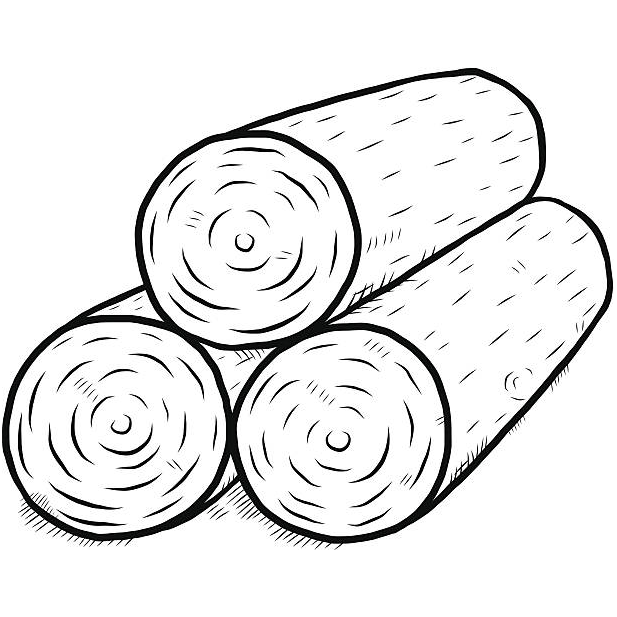
\includegraphics[height=0.6cm]{img/lumber.png}}
        \end{minipage}\\[\BCRuleSpace]
		
		%% Settlement
		\vrule width \textwidth height 2pt \\[\BCRuleSpace]
		\begin{minipage}{2cm}
		    \raggedright
            Settlement \\ \tiny{\quad = 1\enspace VP}
        \end{minipage}
        \hfill
        \begin{minipage}{4cm}
        \raggedleft
            \fbox{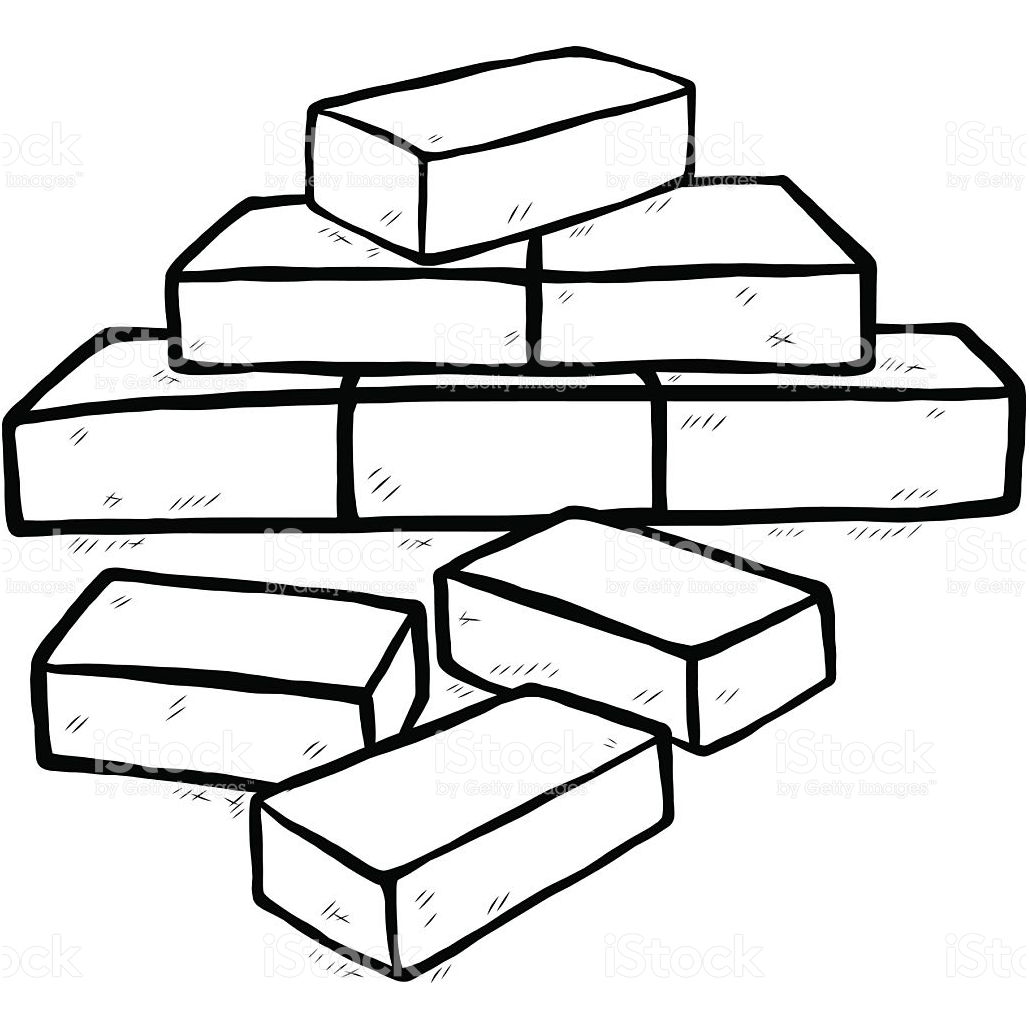
\includegraphics[height=0.6cm]{img/bricks.png}}
            \fbox{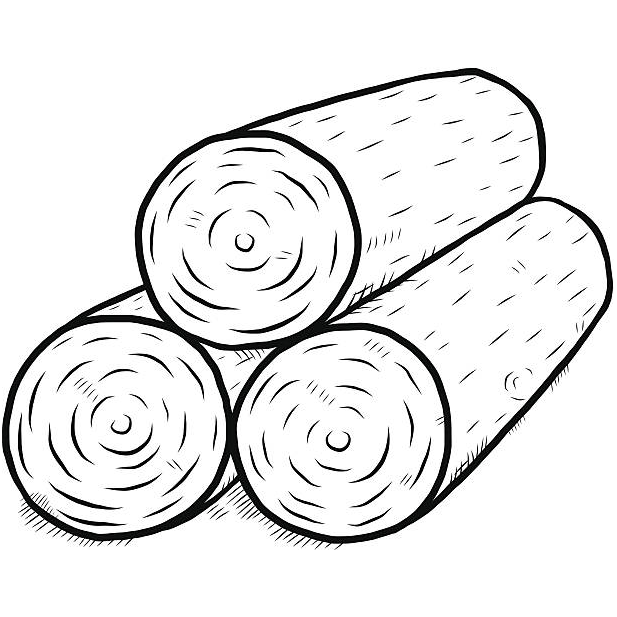
\includegraphics[height=0.6cm]{img/lumber.png}}
		    \fbox{
\includegraphics[height=0.6cm]{img/wheat.png}}
		    \fbox{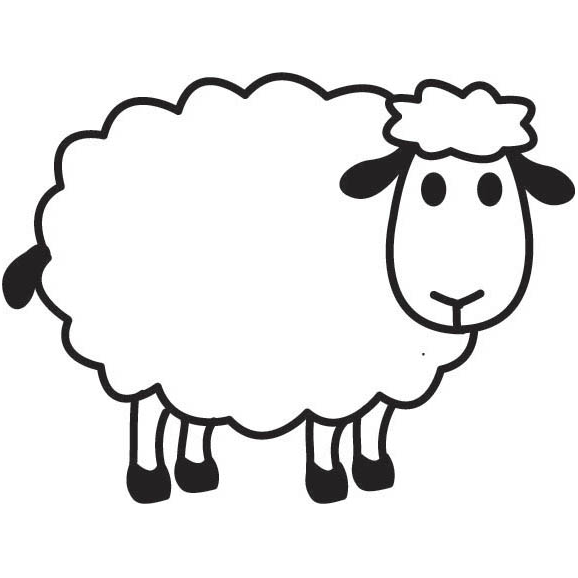
\includegraphics[height=0.6cm]{img/sheep.png}}
        \end{minipage}\\[\BCRuleSpace]
        
        %% City
        \vrule width \textwidth height 2pt \\[\BCRuleSpace]
		\begin{minipage}{1.2cm}
		    \raggedright
            City \\ \tiny{\quad = 2\enspace VP}
        \end{minipage}
        \hfill
        \begin{minipage}{5cm}
        \raggedleft
            \fbox{
\includegraphics[height=0.6cm]{img/wheat.png}}
		    \fbox{
\includegraphics[height=0.6cm]{img/wheat.png}}
		    \fbox{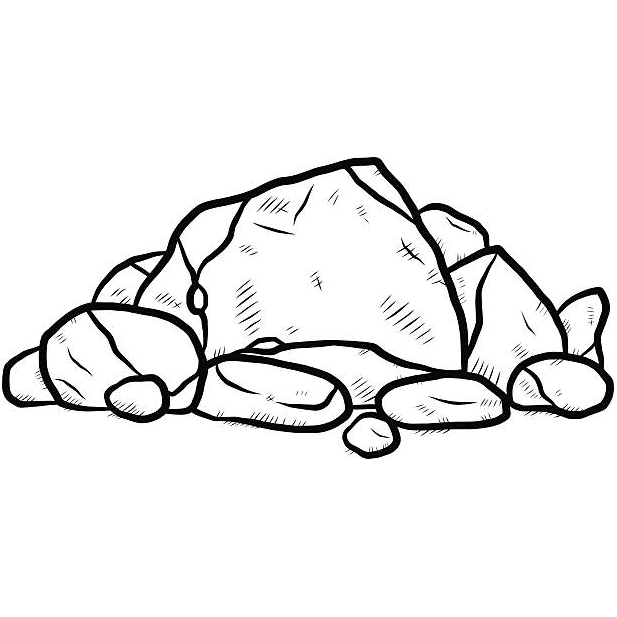
\includegraphics[height=0.6cm]{img/rocks.png}}
		    \fbox{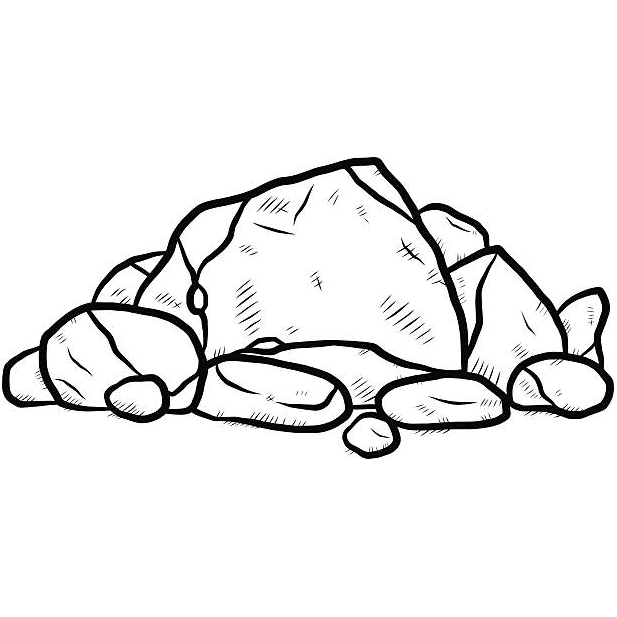
\includegraphics[height=0.6cm]{img/rocks.png}}
		    \fbox{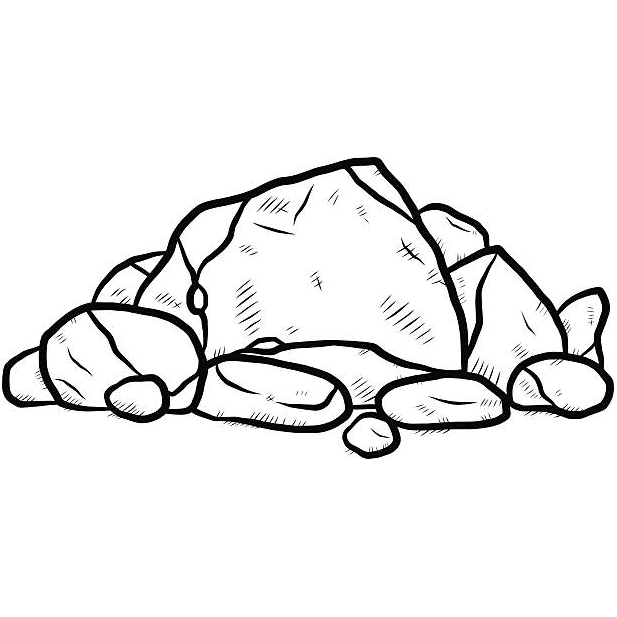
\includegraphics[height=0.6cm]{img/rocks.png}}
        \end{minipage}\\[\BCRuleSpace]
		
		%% Development Card
		\vrule width \textwidth height 2pt \\[\BCRuleSpace]
		\begin{minipage}{3cm}
		    \raggedright
            Development \\[2pt] Card \tiny{\quad = ?\enspace VP}
        \end{minipage}
        \hfill
        \begin{minipage}{3cm}
        \raggedleft
            \fbox{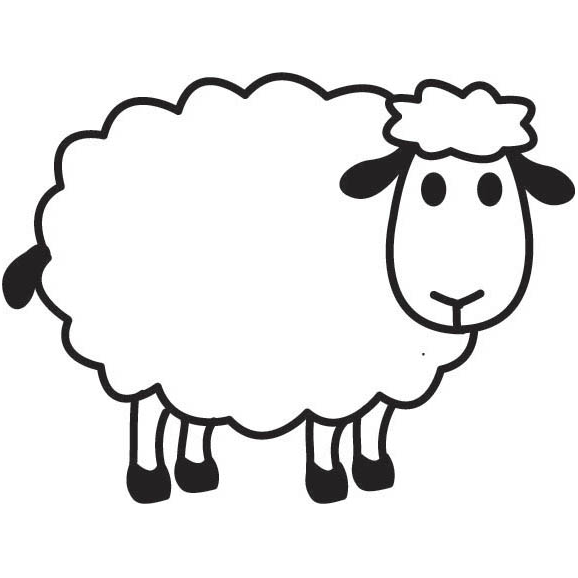
\includegraphics[height=0.6cm]{img/sheep.png}}
		    \fbox{
\includegraphics[height=0.6cm]{img/wheat.png}}
		    \fbox{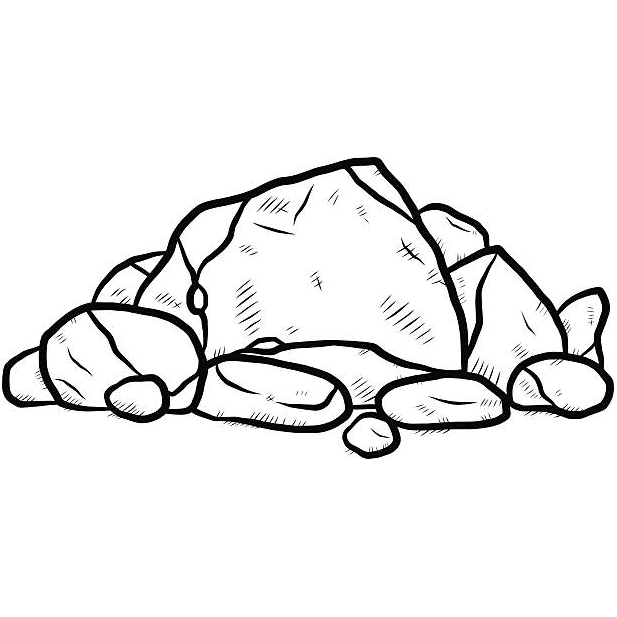
\includegraphics[height=0.6cm]{img/rocks.png}}
        \end{minipage}\\[\BCRuleSpace]
		
		\vrule width \textwidth height 2pt \\[40pt]
		
		%% Extra info
		{\footnotesize
		A player is only allowed to play \textbf{one} development card per turn.\\[10pt]
% 		You can build and trade as much as you like and are able to, and you can do the operations in any order.

        \textbf{On dice-roll 7:} All players with more than 7 cards discards half (rounded down), move the robber to a new tile, and take one resource card from one player with a settlement on the new tile, No development cards can be stolen.
		}
	}

	       % \cardprice{35}
	\cardtypeRule{Building costs}
	\cardborder
	\end{tikzpicture}
}


%%%   Resources   %%%
\newcommand{\resource}[2]{
	\begin{tikzpicture}
	\cardtitle{#2}
	\cardresource{#1}
	\cardborder
	%       \carddebug
	\end{tikzpicture}
}
\newcommand{\lumber}{\resource{img/lumber.png}{Lumber}}
\newcommand{\wool}{\resource{img/sheep.png}{Wool}}
\newcommand{\grain}{\resource{img/wheat.png}{Grain}}
\newcommand{\brick}{\resource{img/bricks.png}{Brick}}
\newcommand{\stone}{\resource{img/rocks.png}{Ore}}

%%%   Development cards   %%%

\newcommand{\knight}{
\begin{tikzpicture}
\devImg{img/knight.png}
%       \carddebug
%		\cardtypeItem
%        \cardtypeAbility
%		\cardtypeTest
%		\cardtypeCharacter
\cardtitle{Knight}
\carddescriptor{Move the robber. \\ \vspace{5mm}Steal \textbf{1} resource from the owner of a settlement or city adjacent to the robber's new hex.}
%        \cardprice{35}
\cardborder
\end{tikzpicture}
}

\newcommand{\road}{
	\begin{tikzpicture}
	\devImg{img/roads.png}
	%       \carddebug
	%		\cardtypeItem
	%        \cardtypeAbility
	%		\cardtypeTest
	%		\cardtypeCharacter
	\cardtitle{Road Building}
	\carddescriptor{Place \textbf{2} new roads as if you had just built them.}
	%        \cardprice{35}
	\cardborder
	\end{tikzpicture}
}

\newcommand{\plenty}{
	\begin{tikzpicture}
	\devImg{img/harvest.png}
	%       \carddebug
	%		\cardtypeItem
	%        \cardtypeAbility
	%		\cardtypeTest
	%		\cardtypeCharacter
	\cardtitle{Year of Plenty}
	\carddescriptor{Take any \textbf{2} resources from the bank. Add them to your hand.\\ They can be 2 of the same resource or 2 different resources.}
	%        \cardprice{35}
	\cardborder
	\end{tikzpicture}
}

\newcommand{\monopoly}{
	\begin{tikzpicture}
	\devImg{img/monopoly.png}
	\cardtitle{Monopoly}
	\carddescriptor{When you play this card, announce \textbf{1 type} of resource.\\ All other players must give you \textbf{all} of their resources of that type.}
	\cardborder
	\end{tikzpicture}
}

\newcommand{\onevp}[2]{
	\begin{tikzpicture}
	\devImg{#2}
	\cardtitle{#1}
	\carddescriptor{\centering\textbf{\Large 1 Victory Point!}\\ \vspace{5mm}Reveal this card on your turn if, with it, you reach the number of points required for victory.}
	\cardborder
	\end{tikzpicture}
}

\newcommand{\chapel}{
	\onevp{Chapel}{img/chapel.jpg}
}

\newcommand{\university}{
	\onevp{University}{img/school.png}
}
\newcommand{\ghall}{
	\onevp{Great Hall}{img/hall.jpg}
}
\newcommand{\library}{
	\onevp{Library}{img/library.png}
}
\newcommand{\market}{
	\onevp{Market}{img/market.jpg}
}

\newcommand{\bonusKnight}{
	\begin{tikzpicture}
	\cardBonusImg{img/largest_army.png}
	\carddescriptor{\centering\textbf{\Large Largest Army \\ \normalsize 2 Victory Points!}\\ \vspace{3mm}\small The first player to play 3 Knight cards gets this card. Another player who plays more knight cards takes this card.}
	\cardtypeBonus{Largest Army}
	\cardborder
	\end{tikzpicture}
}
\newcommand{\bonusRoad}{
	\begin{tikzpicture}
	\cardBonusImg{img/long_road.jpg}
	\carddescriptor{\centering\textbf{\Large Longest Road \\ \normalsize 2 Victory Points!}\\ \vspace{3mm}\small This card goes to the player with the longest unbroken road of at least 5 segments. Another player who builds a longer road takes this card.}
	\cardtypeBonus{Longest Road}
	\cardborder
	\end{tikzpicture}
}

